\begin{event}{Workshop on Data in Mathematics}{math-data-w}{Cernay, France, August 17th to 24th}{PS, FAU}{14}{11}{https://opendreamkit.org/2019/08/17/WorkshopOnDataInMathematics/}

\textbf{Main goals.} 

\textbf{ODK implication.} This event was organized and funded by OpenDreamKit (Paris Sud, FAU). 
OpenDreamKit funded accommodation for all participants, as well as travel expenses for all but two.

\textbf{Event summary.} This workshop brought together interested users and authors of mathematical datasets, 
data framework developers, and experts interested in integrating mathematical databases with computer algebra systems.
Participants discussed general issues related to data in mathematics,
as well as working on concrete steps towards improving the status.

\textbf{Demographic.} The workshop was attended by 
two PhD students,
a postdoc,
four research software engineers,
and seven researchers from various areas of mathematics and computer science.

\textbf{Results and impact.} 
The workshop allowed for a lot of time for free discussion.
Several pain points experienced by mathematicians that work with data came up this way,
were noted, and several cases already acted upon.
In particular, there appears to be a real need for a journal dedicated to 
mathematical datasets and mathematical software.

Discussions on provenance of data in mathematics,
initiated by Dr. Michael Kohlhase, resulted in 
a draft of a standard and formalisation of math data provenance.

Similarly, participants collaborated on how the web interface
for datasets in mathematics should look like.
This effort was led by Dr. Andrea Kohlhase and resulted in 
a clickable prototype in addition to a long list of requirements,
sorted into must--have, should--have, and can't--have.

Participants from FAU are working on an infrastructure for math data and
significant effort went into improving this prototype system.
As planned, we were able to import several real-life datasets.
This included writing up descriptions, metadata (including provenance), 
formalising the mathematics.
In addition to the datasets that were planned for import,
several participants identified the need for new datasets for their 
research communities, and have started to work on them.
The diverse backgrounds of the participants made for a helpful
environment for this.

Participants also worked on side projects related to data in mathematics.
Odile Bénassy was able to quickly produce a basic Jupyter interface to the system,
opening up new interface possibilities.
Several user stories were collected by Gabe Cunningham, and will serve as use cases for the system.
Participants also added content to a multilingual math glossary.

The following testimonials indicate the degree of progress made in a single week.

\begin{quote}
Gabe Cunningham

\emph{``By bringing together the developers of the MathHub with the mathematicians who are producing and analyzing math data, the workshop accomplished in a week what would have otherwise taken months. It was immensely gratifying to see how quickly the system evolved into something that is already better than the state of the art for most mathematicians.''}
\end{quote}
\vspace{5mm}

\begin{quote}
Andrea Kohlhase

\emph{``We had a super intense workshop with people with very different, complementing competencies all strongly willing to work together towards the same goal of pushing the data on MathHub idea: a real team evolved and with that a push beyond my expectations.''}
\end{quote}
\vspace{5mm}

\begin{quote}
Jukka Kohonen

\emph{``For me this was a great way of getting to know people working towards open math data. It was also an opportunity to see the general idea from different perspectives, including concrete databases, user interfaces, and formal and informal logic interconnecting the data. All this and good concrete steps taken within a superbly leisurely setting -- I was absolutely enjoying my time!''}
\end{quote}


\begin{figure}[ht]
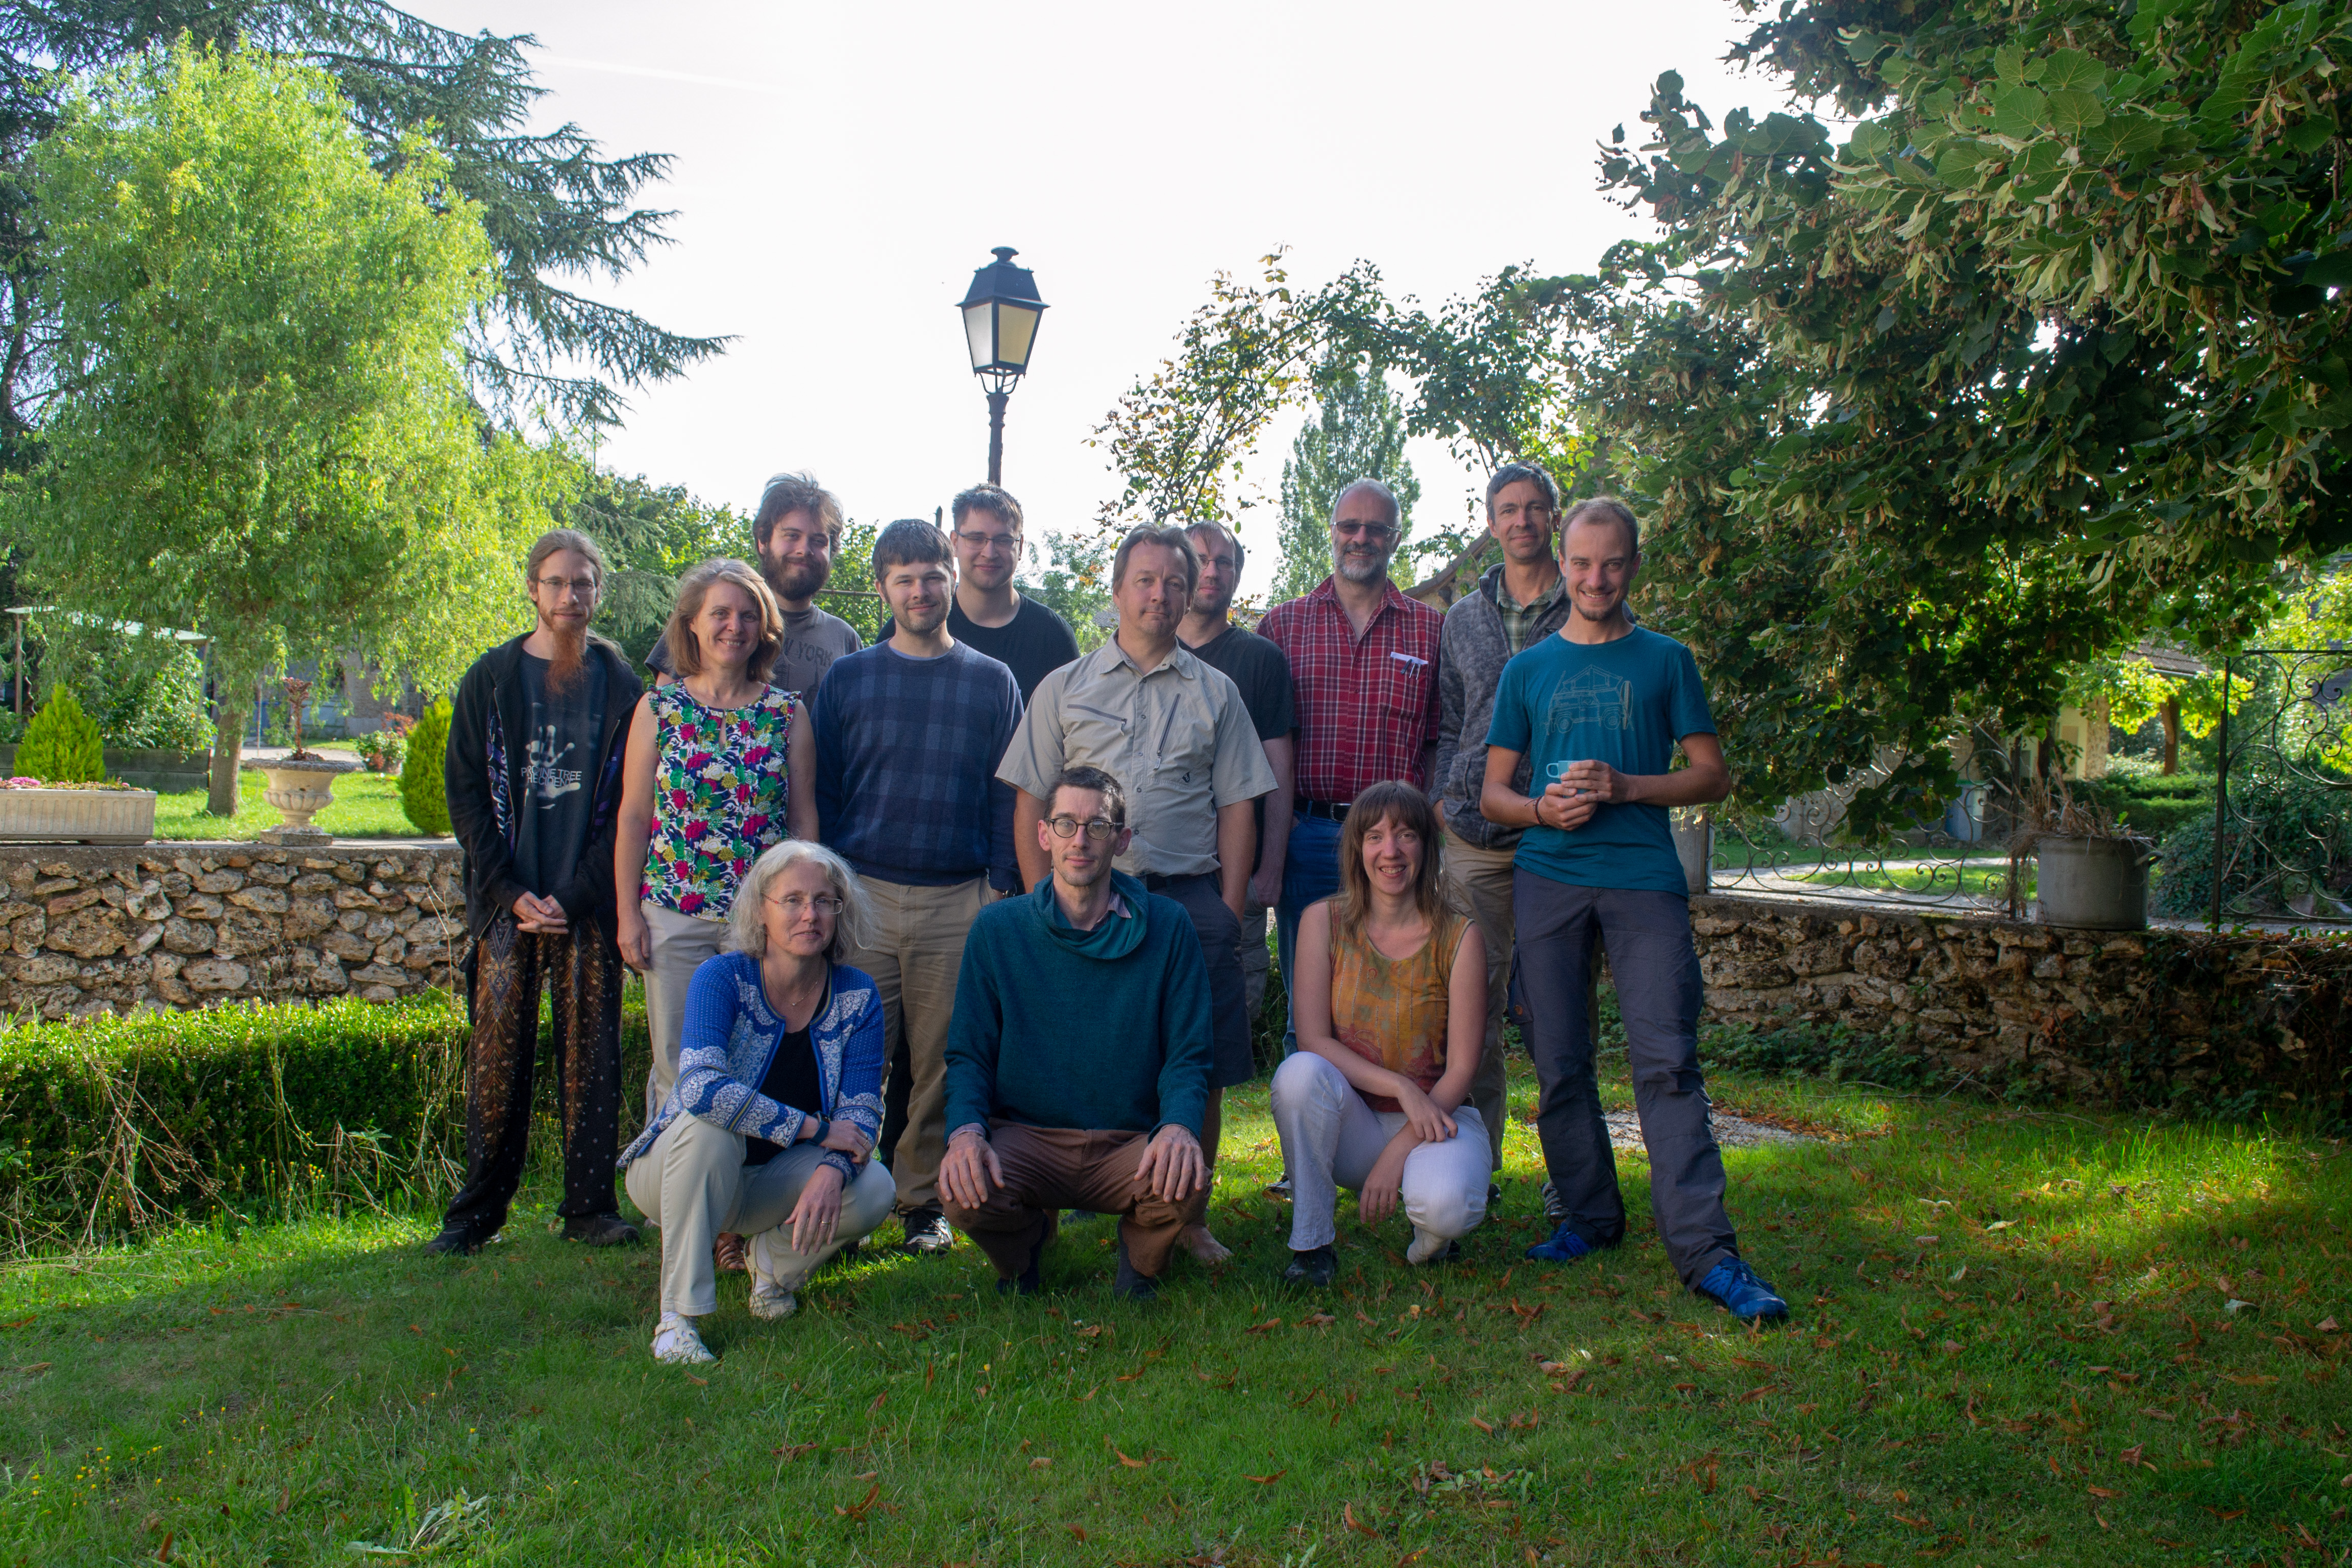
\includegraphics[scale=0.3]{math-data.jpg}
\caption*{Workshop on Data in Mathematics, Cernay, France}
\end{figure}

\end{event}
